% This work is made available under the terms of the
% Creative Commons Attribution-ShareAlike 4.0 license,
% http://creativecommons.org/licenses/by-sa/4.0/.

\documentclass[a4paper]{book}

\usepackage{wrapfig}
\usepackage{graphicx}
\usepackage{hyperref}
\usepackage{multirow}
\usepackage{scalefnt}
\usepackage{tikz}

% watermark -- for draft stage
%\usepackage[firstpage]{draftwatermark}
%\SetWatermarkLightness{0.9}
%\SetWatermarkScale{5}

% Copyright (c) 2009 by the University of Waikato, Hamilton, NZ. 
% This work is made available under the terms of the 
% Creative Commons Attribution-ShareAlike 4.0 license,
% http://creativecommons.org/licenses/by-sa/4.0/.
%
% Version: $Revision: 13214 $

\newenvironment{tight_itemize}{
\begin{itemize}
  \setlength{\itemsep}{1pt}
  \setlength{\parskip}{0pt}
  \setlength{\parsep}{0pt}}{\end{itemize}
}

\newenvironment{tight_enumerate}{
\begin{enumerate}
  \setlength{\itemsep}{1pt}
  \setlength{\parskip}{0pt}
  \setlength{\parsep}{0pt}}{\end{enumerate}
}

% if you just need a simple heading
% Usage:
%   \heading{the text of the heading}
\newcommand{\heading}[1]{
  \vspace{0.3cm} \noindent \textbf{#1} \newline
}

\newcommand{\icon}[1]{\tikz[baseline=-3pt]\node[inner sep=0pt,outer sep=0pt]{\includegraphics[height=1.1em]{#1}};}


\title{
  \textbf{ADAMS} \\
  {\Large \textbf{A}dvanced \textbf{D}ata mining \textbf{A}nd \textbf{M}achine
  learning \textbf{S}ystem} \\
  {\Large Module: adams-ufdl-speech} \\
  \vspace{1cm}
  
\includegraphics[width=2cm]{images/ufdl-speech-module.png} \\
}
\author{
  Peter Reutemann
}

\setcounter{secnumdepth}{3}
\setcounter{tocdepth}{3}

\begin{document}

\begin{titlepage}
\maketitle

\thispagestyle{empty}
\center
\begin{table}[b]
	\begin{tabular}{c l l}
		\parbox[c][2cm]{2cm}{\copyright 2020} &
		\parbox[c][2cm]{5cm}{
\includegraphics[width=5cm]{images/coat_of_arms.pdf}} \\
	\end{tabular}
	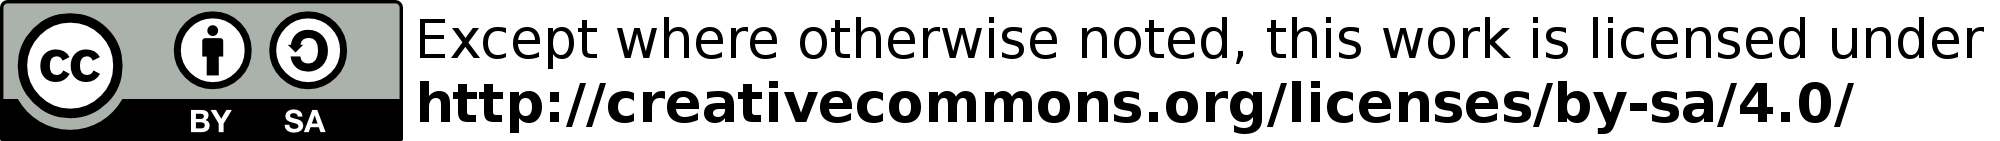
\includegraphics[width=12cm]{images/cc.png} \\
\end{table}

\end{titlepage}

\tableofcontents
%\listoffigures
%\listoftables

%%%%%%%%%%%%%%%%%%%%%%%%%%%%%%%%%%%
\chapter{UFDL}
UFDL, or user-friendly deep-learning, enables users with little or no deep-learning
expertise to maintain datasets for deep-learning tasks such as speech
and object detection and also build deep-learnings models using these.

This ADAMS module focuses on speech processing tasks.

%%%%%%%%%%%%%%%%%%%%%%%%%%%%%%%%%%%
\chapter{Flow}

In addition to the core UFDL components, you also have the following ones available.
These are used in the management flow \textit{adams-ufdl-speech-manage\_speech\_datasets.flow},
which can be used for administrating speech datasets.

The following conversions are available:
\begin{tight_itemize}
  \item \textit{UFDLSpeechDatasetFilesToSpreadSheet} -- turns the files and transcripts of a speed dataset into a spreadsheet
  \item \textit{UFDLSpeechDatasetToListItem} -- converts a UFDL SpeechDataset to a list item string.
  \item \textit{UFDLSpeechDatasetToSpreadSheet} -- turns a speech dataset into a spreadsheet
\end{tight_itemize}

\section{Actions}
The following sink actions can be used:
\begin{tight_itemize}
  \item \textit{DownloadSpeechDataset} -- downloads a speech dataset
\end{tight_itemize}
The following source actions can be used:
\begin{tight_itemize}
  \item \textit{CreateSpeechDatasets} -- creates a speech dataset
  \item \textit{ListSpeechDatasets} -- lists speech datasets
\end{tight_itemize}
The following transformer actions can be used:
\begin{tight_itemize}
  \item \textit{AddSpeechFile} -- adds files to a speech dataset
  \item \textit{DeleteSpeechDataset} -- removes the specified speech dataset
  \item \textit{DeleteSpeechFile} -- removes the specified files from a speech dataset
  \item \textit{GetSpeechFile} -- retrieves a file from a speech dataset via its name
  \item \textit{GetSpeechMetadataForFile} -- retrieves the metadata for an file of a speech dataset via its name
  \item \textit{GetSpeechTranscripts} -- retrieves the map of file/transcripts for a dataset
  \item \textit{GetSpeechTranscriptForFile} -- retrieves the transcript of a file from a dataset
  \item \textit{ListSpeechFiles} -- lists all the files in a speech dataset
  \item \textit{SetSpeechMetadataForFile} -- sets the metadata of an file in an object detection dataset
  \item \textit{SetSpeechTranscriptForFile} -- sets the metadata of an file in an object detection dataset
\end{tight_itemize}

\section{EnterManyValues extensions}
The following extensions of value definitions used by the \textit{EnterManyValues}
source make it easier for users to select PKs:
\begin{tight_itemize}
  \item \textit{UFDLSpeechDatasetList} -- for selecting a speech dataset
\end{tight_itemize}

%%%%%%%%%%%%%%%%%%%%%%%%%%%%%%%%%%%
% This work is made available under the terms of the 
% Creative Commons Attribution-ShareAlike 4.0 license,
% http://creativecommons.org/licenses/by-sa/4.0/.
%
% Version: $Revision: 13411 $

\begin{thebibliography}{999}
	% to make the bibliography appear in the TOC
	\addcontentsline{toc}{chapter}{Bibliography}

    % references
	\bibitem{adams}
		\textit{ADAMS} -- Advanced Data mining and Machine learning System \\
		\url{https://adams.cms.waikato.ac.nz/}{}

\end{thebibliography}


\end{document}
